\documentclass[1p]{elsarticle_modified}
%\bibliographystyle{elsarticle-num}

%\usepackage[colorlinks]{hyperref}
%\usepackage{abbrmath_seonhwa} %\Abb, \Ascr, \Acal ,\Abf, \Afrak
\usepackage{amsfonts}
\usepackage{amssymb}
\usepackage{amsmath}
\usepackage{amsthm}
\usepackage{scalefnt}
\usepackage{amsbsy}
\usepackage{kotex}
\usepackage{caption}
\usepackage{subfig}
\usepackage{color}
\usepackage{graphicx}
\usepackage{xcolor} %% white, black, red, green, blue, cyan, magenta, yellow
\usepackage{float}
\usepackage{setspace}
\usepackage{hyperref}

\usepackage{tikz}
\usetikzlibrary{arrows}

\usepackage{multirow}
\usepackage{array} % fixed length table
\usepackage{hhline}

%%%%%%%%%%%%%%%%%%%%%
\makeatletter
\renewcommand*\env@matrix[1][\arraystretch]{%
	\edef\arraystretch{#1}%
	\hskip -\arraycolsep
	\let\@ifnextchar\new@ifnextchar
	\array{*\c@MaxMatrixCols c}}
\makeatother %https://tex.stackexchange.com/questions/14071/how-can-i-increase-the-line-spacing-in-a-matrix
%%%%%%%%%%%%%%%

\usepackage[normalem]{ulem}

\newcommand{\msout}[1]{\ifmmode\text{\sout{\ensuremath{#1}}}\else\sout{#1}\fi}
%SOURCE: \msout is \stkout macro in https://tex.stackexchange.com/questions/20609/strikeout-in-math-mode

\newcommand{\cancel}[1]{
	\ifmmode
	{\color{red}\msout{#1}}
	\else
	{\color{red}\sout{#1}}
	\fi
}

\newcommand{\add}[1]{
	{\color{blue}\uwave{#1}}
}

\newcommand{\replace}[2]{
	\ifmmode
	{\color{red}\msout{#1}}{\color{blue}\uwave{#2}}
	\else
	{\color{red}\sout{#1}}{\color{blue}\uwave{#2}}
	\fi
}

\newcommand{\Sol}{\mathcal{S}} %segment
\newcommand{\D}{D} %diagram
\newcommand{\A}{\mathcal{A}} %arc


%%%%%%%%%%%%%%%%%%%%%%%%%%%%%5 test

\def\sl{\operatorname{\textup{SL}}(2,\Cbb)}
\def\psl{\operatorname{\textup{PSL}}(2,\Cbb)}
\def\quan{\mkern 1mu \triangleright \mkern 1mu}

\theoremstyle{definition}
\newtheorem{thm}{Theorem}[section]
\newtheorem{prop}[thm]{Proposition}
\newtheorem{lem}[thm]{Lemma}
\newtheorem{ques}[thm]{Question}
\newtheorem{cor}[thm]{Corollary}
\newtheorem{defn}[thm]{Definition}
\newtheorem{exam}[thm]{Example}
\newtheorem{rmk}[thm]{Remark}
\newtheorem{alg}[thm]{Algorithm}

\newcommand{\I}{\sqrt{-1}}
\begin{document}

%\begin{frontmatter}
%
%\title{Boundary parabolic representations of knots up to 8 crossings}
%
%%% Group authors per affiliation:
%\author{Yunhi Cho} 
%\address{Department of Mathematics, University of Seoul, Seoul, Korea}
%\ead{yhcho@uos.ac.kr}
%
%
%\author{Seonhwa Kim} %\fnref{s_kim}}
%\address{Center for Geometry and Physics, Institute for Basic Science, Pohang, 37673, Korea}
%\ead{ryeona17@ibs.re.kr}
%
%\author{Hyuk Kim}
%\address{Department of Mathematical Sciences, Seoul National University, Seoul 08826, Korea}
%\ead{hyukkim@snu.ac.kr}
%
%\author{Seokbeom Yoon}
%\address{Department of Mathematical Sciences, Seoul National University, Seoul, 08826,  Korea}
%\ead{sbyoon15@snu.ac.kr}
%
%\begin{abstract}
%We find all boundary parabolic representation of knots up to 8 crossings.
%
%\end{abstract}
%\begin{keyword}
%    \MSC[2010] 57M25 
%\end{keyword}
%
%\end{frontmatter}

%\linenumbers
%\tableofcontents
%
\newcommand\colored[1]{\textcolor{white}{\rule[-0.35ex]{0.8em}{1.4ex}}\kern-0.8em\color{red} #1}%
%\newcommand\colored[1]{\textcolor{white}{ #1}\kern-2.17ex	\textcolor{white}{ #1}\kern-1.81ex	\textcolor{white}{ #1}\kern-2.15ex\color{red}#1	}

{\Large $\underline{11a_{330}~(K11a_{330})}$}

\setlength{\tabcolsep}{10pt}
\renewcommand{\arraystretch}{1.6}
\vspace{1cm}\begin{tabular}{m{100pt}>{\centering\arraybackslash}m{274pt}}
\multirow{5}{120pt}{
	\centering
	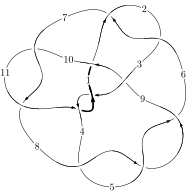
\includegraphics[width=112pt]{../../../GIT/diagram.site/Diagrams/png/579_11a_330.png}\\
\ \ \ A knot diagram\footnotemark}&
\allowdisplaybreaks
\textbf{Linearized knot diagam} \\
\cline{2-2}
 &
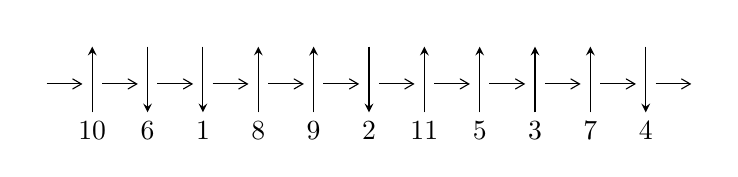
\begin{tikzpicture}[x=20pt, y=17pt]
	% nodes
	\node (C0) at (0, 0) {};
	\node (C1) at (1, 0) {};
	\node (C1U) at (1, +1) {};
	\node (C1D) at (1, -1) {10};

	\node (C2) at (2, 0) {};
	\node (C2U) at (2, +1) {};
	\node (C2D) at (2, -1) {6};

	\node (C3) at (3, 0) {};
	\node (C3U) at (3, +1) {};
	\node (C3D) at (3, -1) {1};

	\node (C4) at (4, 0) {};
	\node (C4U) at (4, +1) {};
	\node (C4D) at (4, -1) {8};

	\node (C5) at (5, 0) {};
	\node (C5U) at (5, +1) {};
	\node (C5D) at (5, -1) {9};

	\node (C6) at (6, 0) {};
	\node (C6U) at (6, +1) {};
	\node (C6D) at (6, -1) {2};

	\node (C7) at (7, 0) {};
	\node (C7U) at (7, +1) {};
	\node (C7D) at (7, -1) {11};

	\node (C8) at (8, 0) {};
	\node (C8U) at (8, +1) {};
	\node (C8D) at (8, -1) {5};

	\node (C9) at (9, 0) {};
	\node (C9U) at (9, +1) {};
	\node (C9D) at (9, -1) {3};

	\node (C10) at (10, 0) {};
	\node (C10U) at (10, +1) {};
	\node (C10D) at (10, -1) {7};

	\node (C11) at (11, 0) {};
	\node (C11U) at (11, +1) {};
	\node (C11D) at (11, -1) {4};
	\node (C12) at (12, 0) {};

	% arrows
	\draw[->,>={angle 60}]
	(C0) edge (C1) (C1) edge (C2) (C2) edge (C3) (C3) edge (C4) (C4) edge (C5) (C5) edge (C6) (C6) edge (C7) (C7) edge (C8) (C8) edge (C9) (C9) edge (C10) (C10) edge (C11) (C11) edge (C12) ;	\draw[->,>=stealth]
	(C1D) edge (C1U) (C2U) edge (C2D) (C3U) edge (C3D) (C4D) edge (C4U) (C5D) edge (C5U) (C6U) edge (C6D) (C7D) edge (C7U) (C8D) edge (C8U) (C9D) edge (C9U) (C10D) edge (C10U) (C11U) edge (C11D) ;
	\end{tikzpicture} \\
\hhline{~~} \\& 
\textbf{Solving Sequence} \\ \cline{2-2} 
 &
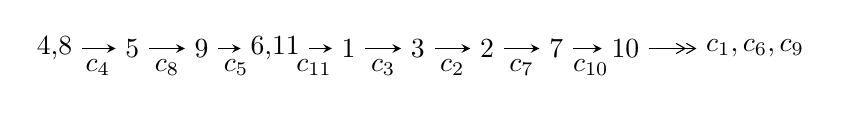
\begin{tikzpicture}[x=25pt, y=7pt]
	% node
	\node (A0) at (-1/8, 0) {4,8};
	\node (A1) at (1, 0) {5};
	\node (A2) at (2, 0) {9};
	\node (A3) at (49/16, 0) {6,11};
	\node (A4) at (33/8, 0) {1};
	\node (A5) at (41/8, 0) {3};
	\node (A6) at (49/8, 0) {2};
	\node (A7) at (57/8, 0) {7};
	\node (A8) at (65/8, 0) {10};
	\node (C1) at (1/2, -1) {$c_{4}$};
	\node (C2) at (3/2, -1) {$c_{8}$};
	\node (C3) at (5/2, -1) {$c_{5}$};
	\node (C4) at (29/8, -1) {$c_{11}$};
	\node (C5) at (37/8, -1) {$c_{3}$};
	\node (C6) at (45/8, -1) {$c_{2}$};
	\node (C7) at (53/8, -1) {$c_{7}$};
	\node (C8) at (61/8, -1) {$c_{10}$};
	\node (A9) at (10, 0) {$c_{1},c_{6},c_{9}$};

	% edge
	\draw[->,>=stealth]	
	(A0) edge (A1) (A1) edge (A2) (A2) edge (A3) (A3) edge (A4) (A4) edge (A5) (A5) edge (A6) (A6) edge (A7) (A7) edge (A8) ;
	\draw[->>,>={angle 60}]	
	(A8) edge (A9);
\end{tikzpicture} \\ 

\end{tabular} \\

\footnotetext{
The image of knot diagram is generated by the software ``\textbf{Draw programme}" developed by Andrew Bartholomew(\url{http://www.layer8.co.uk/maths/draw/index.htm\#Running-draw}), where we modified some parts for our purpose(\url{https://github.com/CATsTAILs/LinksPainter}).
}\phantom \\ \newline 
\centering \textbf{Ideals for irreducible components\footnotemark of $X_{\text{par}}$} 
 
\begin{align*}
I^u_{1}&=\langle 
-1.12011\times10^{74} u^{58}+2.75629\times10^{74} u^{57}+\cdots+3.44884\times10^{73} b-1.05135\times10^{76},\\
\phantom{I^u_{1}}&\phantom{= \langle  }-1.49619\times10^{76} u^{58}+3.79895\times10^{76} u^{57}+\cdots+1.62096\times10^{75} a-1.57571\times10^{78},\\
\phantom{I^u_{1}}&\phantom{= \langle  }u^{59}-3 u^{58}+\cdots-68 u-47\rangle \\
I^u_{2}&=\langle 
u^{13}- u^{12}-7 u^{11}+8 u^{10}+16 u^9-22 u^8-10 u^7+23 u^6-7 u^5-5 u^4+7 u^3-3 u^2+b- u+1,\\
\phantom{I^u_{2}}&\phantom{= \langle  }- u^{14}+2 u^{13}+\cdots+a+2,\\
\phantom{I^u_{2}}&\phantom{= \langle  }u^{15}-2 u^{14}-7 u^{13}+16 u^{12}+15 u^{11}-46 u^{10}-3 u^9+54 u^8-25 u^7-16 u^6+26 u^5-12 u^4-6 u^3+7 u^2-2 u-1\rangle \\
\\
\end{align*}
\raggedright * 2 irreducible components of $\dim_{\mathbb{C}}=0$, with total 74 representations.\\
\footnotetext{All coefficients of polynomials are rational numbers. But the coefficients are sometimes approximated in decimal forms when there is not enough margin.}
\newpage
\renewcommand{\arraystretch}{1}
\centering \section*{I. $I^u_{1}= \langle -1.12\times10^{74} u^{58}+2.76\times10^{74} u^{57}+\cdots+3.45\times10^{73} b-1.05\times10^{76},\;-1.50\times10^{76} u^{58}+3.80\times10^{76} u^{57}+\cdots+1.62\times10^{75} a-1.58\times10^{78},\;u^{59}-3 u^{58}+\cdots-68 u-47 \rangle$}
\flushleft \textbf{(i) Arc colorings}\\
\begin{tabular}{m{7pt} m{180pt} m{7pt} m{180pt} }
\flushright $a_{4}=$&$\begin{pmatrix}1\\0\end{pmatrix}$ \\
\flushright $a_{8}=$&$\begin{pmatrix}0\\u\end{pmatrix}$ \\
\flushright $a_{5}=$&$\begin{pmatrix}1\\- u^2\end{pmatrix}$ \\
\flushright $a_{9}=$&$\begin{pmatrix}u\\- u^3+u\end{pmatrix}$ \\
\flushright $a_{6}=$&$\begin{pmatrix}- u^2+1\\u^4-2 u^2\end{pmatrix}$ \\
\flushright $a_{11}=$&$\begin{pmatrix}9.23031 u^{58}-23.4365 u^{57}+\cdots+3493.41 u+972.086\\3.24779 u^{58}-7.99193 u^{57}+\cdots+1122.55 u+304.842\end{pmatrix}$ \\
\flushright $a_{1}=$&$\begin{pmatrix}5.98251 u^{58}-15.4445 u^{57}+\cdots+2370.86 u+667.245\\3.24779 u^{58}-7.99193 u^{57}+\cdots+1122.55 u+304.842\end{pmatrix}$ \\
\flushright $a_{3}=$&$\begin{pmatrix}2.41804 u^{58}-6.03112 u^{57}+\cdots+1112.39 u+331.970\\3.35170 u^{58}-8.54361 u^{57}+\cdots+1242.14 u+331.682\end{pmatrix}$ \\
\flushright $a_{2}=$&$\begin{pmatrix}5.18004 u^{58}-13.0960 u^{57}+\cdots+2212.35 u+639.499\\2.03204 u^{58}-5.19353 u^{57}+\cdots+732.562 u+188.668\end{pmatrix}$ \\
\flushright $a_{7}=$&$\begin{pmatrix}3.24999 u^{58}-7.66870 u^{57}+\cdots+1187.04 u+318.226\\2.73447 u^{58}-7.36256 u^{57}+\cdots+1055.99 u+271.177\end{pmatrix}$ \\
\flushright $a_{10}=$&$\begin{pmatrix}-0.648359 u^{58}+1.03490 u^{57}+\cdots+370.690 u+121.526\\2.37556 u^{58}-5.68960 u^{57}+\cdots+673.282 u+160.207\end{pmatrix}$\\ \flushright $a_{10}=$&$\begin{pmatrix}-0.648359 u^{58}+1.03490 u^{57}+\cdots+370.690 u+121.526\\2.37556 u^{58}-5.68960 u^{57}+\cdots+673.282 u+160.207\end{pmatrix}$\\&\end{tabular}
\flushleft \textbf{(ii) Obstruction class $= -1$}\\~\\
\flushleft \textbf{(iii) Cusp Shapes $= -19.2036 u^{58}+48.6512 u^{57}+\cdots-6597.80 u-1810.72$}\\~\\
\newpage\renewcommand{\arraystretch}{1}
\flushleft \textbf{(iv) u-Polynomials at the component}\newline \\
\begin{tabular}{m{50pt}|m{274pt}}
Crossings & \hspace{64pt}u-Polynomials at each crossing \\
\hline $$\begin{aligned}c_{1}\end{aligned}$$&$\begin{aligned}
&u^{59}+8 u^{58}+\cdots+7075 u+1561
\end{aligned}$\\
\hline $$\begin{aligned}c_{2},c_{6}\end{aligned}$$&$\begin{aligned}
&u^{59}+2 u^{58}+\cdots- u+1
\end{aligned}$\\
\hline $$\begin{aligned}c_{3},c_{11}\end{aligned}$$&$\begin{aligned}
&u^{59}-3 u^{58}+\cdots-44 u+1
\end{aligned}$\\
\hline $$\begin{aligned}c_{4},c_{5},c_{8}\end{aligned}$$&$\begin{aligned}
&u^{59}-3 u^{58}+\cdots-68 u-47
\end{aligned}$\\
\hline $$\begin{aligned}c_{7},c_{10}\end{aligned}$$&$\begin{aligned}
&u^{59}-30 u^{57}+\cdots+331 u-19
\end{aligned}$\\
\hline $$\begin{aligned}c_{9}\end{aligned}$$&$\begin{aligned}
&u^{59}-2 u^{58}+\cdots+2319 u+2117
\end{aligned}$\\
\hline
\end{tabular}\\~\\
\newpage\renewcommand{\arraystretch}{1}
\flushleft \textbf{(v) Riley Polynomials at the component}\newline \\
\begin{tabular}{m{50pt}|m{274pt}}
Crossings & \hspace{64pt}Riley Polynomials at each crossing \\
\hline $$\begin{aligned}c_{1}\end{aligned}$$&$\begin{aligned}
&y^{59}-28 y^{58}+\cdots+51101495 y-2436721
\end{aligned}$\\
\hline $$\begin{aligned}c_{2},c_{6}\end{aligned}$$&$\begin{aligned}
&y^{59}+48 y^{58}+\cdots+143 y-1
\end{aligned}$\\
\hline $$\begin{aligned}c_{3},c_{11}\end{aligned}$$&$\begin{aligned}
&y^{59}+51 y^{58}+\cdots+564 y-1
\end{aligned}$\\
\hline $$\begin{aligned}c_{4},c_{5},c_{8}\end{aligned}$$&$\begin{aligned}
&y^{59}-69 y^{58}+\cdots+52564 y-2209
\end{aligned}$\\
\hline $$\begin{aligned}c_{7},c_{10}\end{aligned}$$&$\begin{aligned}
&y^{59}-60 y^{58}+\cdots+84595 y-361
\end{aligned}$\\
\hline $$\begin{aligned}c_{9}\end{aligned}$$&$\begin{aligned}
&y^{59}-32 y^{58}+\cdots+164317887 y-4481689
\end{aligned}$\\
\hline
\end{tabular}\\~\\
\newpage\flushleft \textbf{(vi) Complex Volumes and Cusp Shapes}
$$\begin{array}{c|c|c}  
\text{Solutions to }I^u_{1}& \I (\text{vol} + \sqrt{-1}CS) & \text{Cusp shape}\\
 \hline 
\begin{aligned}
u &= \phantom{-}0.663884 + 0.670936 I \\
a &= -1.15868 + 0.88811 I \\
b &= -0.33009 + 1.44308 I\end{aligned}
 & \phantom{-}5.56188 + 5.09196 I & \phantom{-0.000000 } 0 \\ \hline\begin{aligned}
u &= \phantom{-}0.663884 - 0.670936 I \\
a &= -1.15868 - 0.88811 I \\
b &= -0.33009 - 1.44308 I\end{aligned}
 & \phantom{-}5.56188 - 5.09196 I & \phantom{-0.000000 } 0 \\ \hline\begin{aligned}
u &= -1.072730 + 0.002898 I \\
a &= -0.708113 + 0.180531 I \\
b &= -0.679774 - 0.774687 I\end{aligned}
 & \phantom{-}1.97600 - 2.55273 I & \phantom{-0.000000 } 0 \\ \hline\begin{aligned}
u &= -1.072730 - 0.002898 I \\
a &= -0.708113 - 0.180531 I \\
b &= -0.679774 + 0.774687 I\end{aligned}
 & \phantom{-}1.97600 + 2.55273 I & \phantom{-0.000000 } 0 \\ \hline\begin{aligned}
u &= \phantom{-}0.481157 + 0.783711 I \\
a &= \phantom{-}0.87764 - 1.18816 I \\
b &= -0.033355 - 1.312050 I\end{aligned}
 & \phantom{-}4.90675 - 0.17949 I & \phantom{-0.000000 } 0 \\ \hline\begin{aligned}
u &= \phantom{-}0.481157 - 0.783711 I \\
a &= \phantom{-}0.87764 + 1.18816 I \\
b &= -0.033355 + 1.312050 I\end{aligned}
 & \phantom{-}4.90675 + 0.17949 I & \phantom{-0.000000 } 0 \\ \hline\begin{aligned}
u &= \phantom{-}0.912889 + 0.065447 I \\
a &= \phantom{-}0.654408 + 0.408442 I \\
b &= -0.109027 - 0.587707 I\end{aligned}
 & \phantom{-}1.58471 + 0.10901 I & \phantom{-0.000000 } 0 \\ \hline\begin{aligned}
u &= \phantom{-}0.912889 - 0.065447 I \\
a &= \phantom{-}0.654408 - 0.408442 I \\
b &= -0.109027 + 0.587707 I\end{aligned}
 & \phantom{-}1.58471 - 0.10901 I & \phantom{-0.000000 } 0 \\ \hline\begin{aligned}
u &= \phantom{-}0.547371 + 0.629034 I \\
a &= \phantom{-}0.275474 + 0.246041 I \\
b &= \phantom{-}0.362689 + 1.069460 I\end{aligned}
 & \phantom{-}4.32344 - 1.31427 I & \phantom{-}8.87224 + 0. I\phantom{ +0.000000I} \\ \hline\begin{aligned}
u &= \phantom{-}0.547371 - 0.629034 I \\
a &= \phantom{-}0.275474 - 0.246041 I \\
b &= \phantom{-}0.362689 - 1.069460 I\end{aligned}
 & \phantom{-}4.32344 + 1.31427 I & \phantom{-}8.87224 + 0. I\phantom{ +0.000000I}\\
 \hline 
 \end{array}$$\newpage$$\begin{array}{c|c|c}  
\text{Solutions to }I^u_{1}& \I (\text{vol} + \sqrt{-1}CS) & \text{Cusp shape}\\
 \hline 
\begin{aligned}
u &= -0.655609 + 0.435361 I \\
a &= \phantom{-}1.52726 + 0.50194 I \\
b &= \phantom{-}0.899285 + 0.164244 I\end{aligned}
 & \phantom{-}5.22435 - 5.58403 I & \phantom{-}7.88408 + 6.48040 I \\ \hline\begin{aligned}
u &= -0.655609 - 0.435361 I \\
a &= \phantom{-}1.52726 - 0.50194 I \\
b &= \phantom{-}0.899285 - 0.164244 I\end{aligned}
 & \phantom{-}5.22435 + 5.58403 I & \phantom{-}7.88408 - 6.48040 I \\ \hline\begin{aligned}
u &= \phantom{-}0.566889 + 0.487295 I \\
a &= \phantom{-}1.27041 + 0.78556 I \\
b &= \phantom{-}0.293328 - 1.120330 I\end{aligned}
 & \phantom{-}4.51202 + 5.11815 I & \phantom{-}8.89658 - 7.24819 I \\ \hline\begin{aligned}
u &= \phantom{-}0.566889 - 0.487295 I \\
a &= \phantom{-}1.27041 - 0.78556 I \\
b &= \phantom{-}0.293328 + 1.120330 I\end{aligned}
 & \phantom{-}4.51202 - 5.11815 I & \phantom{-}8.89658 + 7.24819 I \\ \hline\begin{aligned}
u &= -0.462881 + 0.565944 I \\
a &= -0.55152 - 1.59437 I \\
b &= \phantom{-}0.0819864 - 0.0135157 I\end{aligned}
 & \phantom{-}4.44971 + 2.14107 I & \phantom{-}5.59927 + 1.54259 I \\ \hline\begin{aligned}
u &= -0.462881 - 0.565944 I \\
a &= -0.55152 + 1.59437 I \\
b &= \phantom{-}0.0819864 + 0.0135157 I\end{aligned}
 & \phantom{-}4.44971 - 2.14107 I & \phantom{-}5.59927 - 1.54259 I \\ \hline\begin{aligned}
u &= -0.870656 + 0.926885 I \\
a &= \phantom{-}0.986934 + 0.667144 I \\
b &= \phantom{-}0.31968 + 1.41732 I\end{aligned}
 & \phantom{-}10.3757 - 9.8566 I & \phantom{-0.000000 } 0 \\ \hline\begin{aligned}
u &= -0.870656 - 0.926885 I \\
a &= \phantom{-}0.986934 - 0.667144 I \\
b &= \phantom{-}0.31968 - 1.41732 I\end{aligned}
 & \phantom{-}10.3757 + 9.8566 I & \phantom{-0.000000 } 0 \\ \hline\begin{aligned}
u &= \phantom{-}0.415938 + 0.579248 I \\
a &= \phantom{-}0.846887 + 0.499107 I \\
b &= \phantom{-}0.574644 + 0.026281 I\end{aligned}
 & \phantom{-}1.35011 + 1.88524 I & \phantom{-}3.00000 - 3.83760 I \\ \hline\begin{aligned}
u &= \phantom{-}0.415938 - 0.579248 I \\
a &= \phantom{-}0.846887 - 0.499107 I \\
b &= \phantom{-}0.574644 - 0.026281 I\end{aligned}
 & \phantom{-}1.35011 - 1.88524 I & \phantom{-}3.00000 + 3.83760 I\\
 \hline 
 \end{array}$$\newpage$$\begin{array}{c|c|c}  
\text{Solutions to }I^u_{1}& \I (\text{vol} + \sqrt{-1}CS) & \text{Cusp shape}\\
 \hline 
\begin{aligned}
u &= -0.647619 + 0.225990 I \\
a &= \phantom{-}1.90147 + 0.85004 I \\
b &= \phantom{-}0.42877 + 1.41249 I\end{aligned}
 & \phantom{-}9.17648 + 0.45587 I & \phantom{-}13.79187 + 0.50236 I \\ \hline\begin{aligned}
u &= -0.647619 - 0.225990 I \\
a &= \phantom{-}1.90147 - 0.85004 I \\
b &= \phantom{-}0.42877 - 1.41249 I\end{aligned}
 & \phantom{-}9.17648 - 0.45587 I & \phantom{-}13.79187 - 0.50236 I \\ \hline\begin{aligned}
u &= \phantom{-}1.31990\phantom{ +0.000000I} \\
a &= \phantom{-}0.0472574\phantom{ +0.000000I} \\
b &= -0.674808\phantom{ +0.000000I}\end{aligned}
 & \phantom{-}2.77979\phantom{ +0.000000I} & \phantom{-0.000000 } 0 \\ \hline\begin{aligned}
u &= -0.507724 + 1.289270 I \\
a &= -0.303043 - 0.951975 I \\
b &= \phantom{-}0.042705 - 1.359630 I\end{aligned}
 & \phantom{-}9.00112 + 2.68298 I & \phantom{-0.000000 } 0 \\ \hline\begin{aligned}
u &= -0.507724 - 1.289270 I \\
a &= -0.303043 + 0.951975 I \\
b &= \phantom{-}0.042705 + 1.359630 I\end{aligned}
 & \phantom{-}9.00112 - 2.68298 I & \phantom{-0.000000 } 0 \\ \hline\begin{aligned}
u &= -1.44030 + 0.20799 I \\
a &= \phantom{-}0.221441 - 0.421025 I \\
b &= \phantom{-}0.542037 + 0.003122 I\end{aligned}
 & \phantom{-}7.30101 - 4.74836 I & \phantom{-0.000000 } 0 \\ \hline\begin{aligned}
u &= -1.44030 - 0.20799 I \\
a &= \phantom{-}0.221441 + 0.421025 I \\
b &= \phantom{-}0.542037 - 0.003122 I\end{aligned}
 & \phantom{-}7.30101 + 4.74836 I & \phantom{-0.000000 } 0 \\ \hline\begin{aligned}
u &= -0.485094 + 0.213274 I \\
a &= -3.30156 - 0.35475 I \\
b &= \phantom{-}0.001691 - 1.297030 I\end{aligned}
 & \phantom{-}8.58837 - 2.03485 I & \phantom{-}15.0115 + 3.6514 I \\ \hline\begin{aligned}
u &= -0.485094 - 0.213274 I \\
a &= -3.30156 + 0.35475 I \\
b &= \phantom{-}0.001691 + 1.297030 I\end{aligned}
 & \phantom{-}8.58837 + 2.03485 I & \phantom{-}15.0115 - 3.6514 I \\ \hline\begin{aligned}
u &= -0.486013 + 0.140699 I \\
a &= -0.526562 + 0.989442 I \\
b &= -0.351844 - 0.983970 I\end{aligned}
 & \phantom{-}0.77762 - 2.37468 I & -0.58026 + 5.71266 I\\
 \hline 
 \end{array}$$\newpage$$\begin{array}{c|c|c}  
\text{Solutions to }I^u_{1}& \I (\text{vol} + \sqrt{-1}CS) & \text{Cusp shape}\\
 \hline 
\begin{aligned}
u &= -0.486013 - 0.140699 I \\
a &= -0.526562 - 0.989442 I \\
b &= -0.351844 + 0.983970 I\end{aligned}
 & \phantom{-}0.77762 + 2.37468 I & -0.58026 - 5.71266 I \\ \hline\begin{aligned}
u &= -1.50589\phantom{ +0.000000I} \\
a &= \phantom{-}0.891008\phantom{ +0.000000I} \\
b &= \phantom{-}0.701190\phantom{ +0.000000I}\end{aligned}
 & \phantom{-}7.41921\phantom{ +0.000000I} & \phantom{-0.000000 } 0 \\ \hline\begin{aligned}
u &= \phantom{-}0.453128\phantom{ +0.000000I} \\
a &= -2.33221\phantom{ +0.000000I} \\
b &= -1.18104\phantom{ +0.000000I}\end{aligned}
 & \phantom{-}0.221271\phantom{ +0.000000I} & \phantom{-}19.3560\phantom{ +0.000000I} \\ \hline\begin{aligned}
u &= \phantom{-}0.452712\phantom{ +0.000000I} \\
a &= \phantom{-}1.61649\phantom{ +0.000000I} \\
b &= \phantom{-}0.0591731\phantom{ +0.000000I}\end{aligned}
 & \phantom{-}0.981228\phantom{ +0.000000I} & \phantom{-}11.9020\phantom{ +0.000000I} \\ \hline\begin{aligned}
u &= \phantom{-}1.55236 + 0.02522 I \\
a &= -0.133426 - 0.715380 I \\
b &= -0.19113 + 1.40151 I\end{aligned}
 & \phantom{-}7.75920 + 2.91351 I & \phantom{-0.000000 } 0 \\ \hline\begin{aligned}
u &= \phantom{-}1.55236 - 0.02522 I \\
a &= -0.133426 + 0.715380 I \\
b &= -0.19113 - 1.40151 I\end{aligned}
 & \phantom{-}7.75920 - 2.91351 I & \phantom{-0.000000 } 0 \\ \hline\begin{aligned}
u &= \phantom{-}1.56343 + 0.06205 I \\
a &= -1.285730 - 0.513846 I \\
b &= -0.270263 + 1.324280 I\end{aligned}
 & \phantom{-}15.6947 + 3.0236 I & \phantom{-0.000000 } 0 \\ \hline\begin{aligned}
u &= \phantom{-}1.56343 - 0.06205 I \\
a &= -1.285730 + 0.513846 I \\
b &= -0.270263 - 1.324280 I\end{aligned}
 & \phantom{-}15.6947 - 3.0236 I & \phantom{-0.000000 } 0 \\ \hline\begin{aligned}
u &= -1.56748\phantom{ +0.000000I} \\
a &= -0.881028\phantom{ +0.000000I} \\
b &= -1.73811\phantom{ +0.000000I}\end{aligned}
 & \phantom{-}7.31990\phantom{ +0.000000I} & \phantom{-0.000000 } 0 \\ \hline\begin{aligned}
u &= -1.57638 + 0.12949 I \\
a &= \phantom{-}0.436873 - 0.982897 I \\
b &= \phantom{-}0.186350 + 1.361050 I\end{aligned}
 & \phantom{-}11.80620 - 7.29433 I & \phantom{-0.000000 } 0\\
 \hline 
 \end{array}$$\newpage$$\begin{array}{c|c|c}  
\text{Solutions to }I^u_{1}& \I (\text{vol} + \sqrt{-1}CS) & \text{Cusp shape}\\
 \hline 
\begin{aligned}
u &= -1.57638 - 0.12949 I \\
a &= \phantom{-}0.436873 + 0.982897 I \\
b &= \phantom{-}0.186350 - 1.361050 I\end{aligned}
 & \phantom{-}11.80620 + 7.29433 I & \phantom{-0.000000 } 0 \\ \hline\begin{aligned}
u &= -1.58483 + 0.22376 I \\
a &= \phantom{-}0.987123 - 0.209265 I \\
b &= \phantom{-}0.273747 + 1.367090 I\end{aligned}
 & \phantom{-}11.87830 - 3.53773 I & \phantom{-0.000000 } 0 \\ \hline\begin{aligned}
u &= -1.58483 - 0.22376 I \\
a &= \phantom{-}0.987123 + 0.209265 I \\
b &= \phantom{-}0.273747 - 1.367090 I\end{aligned}
 & \phantom{-}11.87830 + 3.53773 I & \phantom{-0.000000 } 0 \\ \hline\begin{aligned}
u &= \phantom{-}1.59540 + 0.14328 I \\
a &= -0.915820 + 0.268097 I \\
b &= -0.698680 + 0.076811 I\end{aligned}
 & \phantom{-}11.68030 + 0.45414 I & \phantom{-0.000000 } 0 \\ \hline\begin{aligned}
u &= \phantom{-}1.59540 - 0.14328 I \\
a &= -0.915820 - 0.268097 I \\
b &= -0.698680 - 0.076811 I\end{aligned}
 & \phantom{-}11.68030 - 0.45414 I & \phantom{-0.000000 } 0 \\ \hline\begin{aligned}
u &= -0.020007 + 0.394814 I \\
a &= -0.649909 + 1.080940 I \\
b &= -0.564266 + 0.401283 I\end{aligned}
 & -0.96759 + 1.06374 I & -3.58491 - 4.50505 I \\ \hline\begin{aligned}
u &= -0.020007 - 0.394814 I \\
a &= -0.649909 - 1.080940 I \\
b &= -0.564266 - 0.401283 I\end{aligned}
 & -0.96759 - 1.06374 I & -3.58491 + 4.50505 I \\ \hline\begin{aligned}
u &= \phantom{-}1.60361 + 0.11834 I \\
a &= \phantom{-}0.911699 + 0.052547 I \\
b &= \phantom{-}1.42194 - 0.25243 I\end{aligned}
 & \phantom{-}12.9698 + 7.5955 I & \phantom{-0.000000 } 0 \\ \hline\begin{aligned}
u &= \phantom{-}1.60361 - 0.11834 I \\
a &= \phantom{-}0.911699 - 0.052547 I \\
b &= \phantom{-}1.42194 + 0.25243 I\end{aligned}
 & \phantom{-}12.9698 - 7.5955 I & \phantom{-0.000000 } 0 \\ \hline\begin{aligned}
u &= \phantom{-}1.60729 + 0.06441 I \\
a &= \phantom{-}0.887442 + 0.078089 I \\
b &= \phantom{-}0.81025 - 1.62623 I\end{aligned}
 & \phantom{-}17.0188 + 0.6284 I & \phantom{-0.000000 } 0\\
 \hline 
 \end{array}$$\newpage$$\begin{array}{c|c|c}  
\text{Solutions to }I^u_{1}& \I (\text{vol} + \sqrt{-1}CS) & \text{Cusp shape}\\
 \hline 
\begin{aligned}
u &= \phantom{-}1.60729 - 0.06441 I \\
a &= \phantom{-}0.887442 - 0.078089 I \\
b &= \phantom{-}0.81025 + 1.62623 I\end{aligned}
 & \phantom{-}17.0188 - 0.6284 I & \phantom{-0.000000 } 0 \\ \hline\begin{aligned}
u &= -1.60407 + 0.19460 I \\
a &= -0.938387 + 0.141608 I \\
b &= -0.58039 - 1.68597 I\end{aligned}
 & \phantom{-}13.1880 - 8.2730 I & \phantom{-0.000000 } 0 \\ \hline\begin{aligned}
u &= -1.60407 - 0.19460 I \\
a &= -0.938387 - 0.141608 I \\
b &= -0.58039 + 1.68597 I\end{aligned}
 & \phantom{-}13.1880 + 8.2730 I & \phantom{-0.000000 } 0 \\ \hline\begin{aligned}
u &= -1.63522 + 0.16039 I \\
a &= \phantom{-}0.003749 + 0.275010 I \\
b &= \phantom{-}0.23042 - 1.41743 I\end{aligned}
 & \phantom{-}12.00310 - 1.72842 I & \phantom{-0.000000 } 0 \\ \hline\begin{aligned}
u &= -1.63522 - 0.16039 I \\
a &= \phantom{-}0.003749 - 0.275010 I \\
b &= \phantom{-}0.23042 + 1.41743 I\end{aligned}
 & \phantom{-}12.00310 + 1.72842 I & \phantom{-0.000000 } 0 \\ \hline\begin{aligned}
u &= \phantom{-}1.68149 + 0.27693 I \\
a &= \phantom{-}1.006940 + 0.127051 I \\
b &= \phantom{-}0.53294 - 1.57371 I\end{aligned}
 & \phantom{-}18.8364 + 14.4187 I & \phantom{-0.000000 } 0 \\ \hline\begin{aligned}
u &= \phantom{-}1.68149 - 0.27693 I \\
a &= \phantom{-}1.006940 - 0.127051 I \\
b &= \phantom{-}0.53294 + 1.57371 I\end{aligned}
 & \phantom{-}18.8364 - 14.4187 I & \phantom{-0.000000 } 0 \\ \hline\begin{aligned}
u &= \phantom{-}1.78123 + 0.42255 I \\
a &= -0.759705 + 0.078407 I \\
b &= -0.27686 + 1.40310 I\end{aligned}
 & \phantom{-}16.5334 + 4.0342 I & \phantom{-0.000000 } 0 \\ \hline\begin{aligned}
u &= \phantom{-}1.78123 - 0.42255 I \\
a &= -0.759705 - 0.078407 I \\
b &= -0.27686 - 1.40310 I\end{aligned}
 & \phantom{-}16.5334 - 4.0342 I & \phantom{-0.000000 } 0\\
 \hline 
 \end{array}$$\newpage\newpage\renewcommand{\arraystretch}{1}
\centering \section*{II. $I^u_{2}= \langle u^{13}- u^{12}+\cdots+b+1,\;- u^{14}+2 u^{13}+\cdots+a+2,\;u^{15}-2 u^{14}+\cdots-2 u-1 \rangle$}
\flushleft \textbf{(i) Arc colorings}\\
\begin{tabular}{m{7pt} m{180pt} m{7pt} m{180pt} }
\flushright $a_{4}=$&$\begin{pmatrix}1\\0\end{pmatrix}$ \\
\flushright $a_{8}=$&$\begin{pmatrix}0\\u\end{pmatrix}$ \\
\flushright $a_{5}=$&$\begin{pmatrix}1\\- u^2\end{pmatrix}$ \\
\flushright $a_{9}=$&$\begin{pmatrix}u\\- u^3+u\end{pmatrix}$ \\
\flushright $a_{6}=$&$\begin{pmatrix}- u^2+1\\u^4-2 u^2\end{pmatrix}$ \\
\flushright $a_{11}=$&$\begin{pmatrix}u^{14}-2 u^{13}+\cdots+6 u-2\\- u^{13}+u^{12}+\cdots+u-1\end{pmatrix}$ \\
\flushright $a_{1}=$&$\begin{pmatrix}u^{14}- u^{13}+\cdots+5 u-1\\- u^{13}+u^{12}+\cdots+u-1\end{pmatrix}$ \\
\flushright $a_{3}=$&$\begin{pmatrix}u^8-5 u^6+u^5+7 u^4-3 u^3- u^2+2 u-1\\- u^{13}+u^{12}+\cdots+u-1\end{pmatrix}$ \\
\flushright $a_{2}=$&$\begin{pmatrix}u^8- u^7-5 u^6+5 u^5+7 u^4-7 u^3- u^2+2 u-2\\- u^{14}+9 u^{12}+\cdots-2 u-2\end{pmatrix}$ \\
\flushright $a_{7}=$&$\begin{pmatrix}- u^{14}+2 u^{13}+\cdots-5 u+2\\- u^{14}+u^{13}+\cdots+3 u^2-2 u\end{pmatrix}$ \\
\flushright $a_{10}=$&$\begin{pmatrix}u^5-3 u^3+2 u\\u^{14}- u^{13}+\cdots+u^2+2 u\end{pmatrix}$\\ \flushright $a_{10}=$&$\begin{pmatrix}u^5-3 u^3+2 u\\u^{14}- u^{13}+\cdots+u^2+2 u\end{pmatrix}$\\&\end{tabular}
\flushleft \textbf{(ii) Obstruction class $= 1$}\\~\\
\flushleft \textbf{(iii) Cusp Shapes $= 3 u^{14}-7 u^{13}-19 u^{12}+53 u^{11}+30 u^{10}-141 u^9+29 u^8+144 u^7-109 u^6-21 u^5+76 u^4-46 u^3-2 u^2+24 u+1$}\\~\\
\newpage\renewcommand{\arraystretch}{1}
\flushleft \textbf{(iv) u-Polynomials at the component}\newline \\
\begin{tabular}{m{50pt}|m{274pt}}
Crossings & \hspace{64pt}u-Polynomials at each crossing \\
\hline $$\begin{aligned}c_{1}\end{aligned}$$&$\begin{aligned}
&u^{15}-3 u^{14}+\cdots+5 u-1
\end{aligned}$\\
\hline $$\begin{aligned}c_{2}\end{aligned}$$&$\begin{aligned}
&u^{15}+u^{14}+\cdots- u-1
\end{aligned}$\\
\hline $$\begin{aligned}c_{3}\end{aligned}$$&$\begin{aligned}
&u^{15}+2 u^{14}+\cdots+2 u+1
\end{aligned}$\\
\hline $$\begin{aligned}c_{4},c_{5}\end{aligned}$$&$\begin{aligned}
&u^{15}-2 u^{14}+\cdots-2 u-1
\end{aligned}$\\
\hline $$\begin{aligned}c_{6}\end{aligned}$$&$\begin{aligned}
&u^{15}- u^{14}+\cdots- u+1
\end{aligned}$\\
\hline $$\begin{aligned}c_{7}\end{aligned}$$&$\begin{aligned}
&u^{15}-3 u^{14}+\cdots+3 u+1
\end{aligned}$\\
\hline $$\begin{aligned}c_{8}\end{aligned}$$&$\begin{aligned}
&u^{15}+2 u^{14}+\cdots-2 u+1
\end{aligned}$\\
\hline $$\begin{aligned}c_{9}\end{aligned}$$&$\begin{aligned}
&u^{15}- u^{14}+\cdots-7 u-1
\end{aligned}$\\
\hline $$\begin{aligned}c_{10}\end{aligned}$$&$\begin{aligned}
&u^{15}+3 u^{14}+\cdots+3 u-1
\end{aligned}$\\
\hline $$\begin{aligned}c_{11}\end{aligned}$$&$\begin{aligned}
&u^{15}-2 u^{14}+\cdots+2 u-1
\end{aligned}$\\
\hline
\end{tabular}\\~\\
\newpage\renewcommand{\arraystretch}{1}
\flushleft \textbf{(v) Riley Polynomials at the component}\newline \\
\begin{tabular}{m{50pt}|m{274pt}}
Crossings & \hspace{64pt}Riley Polynomials at each crossing \\
\hline $$\begin{aligned}c_{1}\end{aligned}$$&$\begin{aligned}
&y^{15}-5 y^{14}+\cdots+13 y-1
\end{aligned}$\\
\hline $$\begin{aligned}c_{2},c_{6}\end{aligned}$$&$\begin{aligned}
&y^{15}+11 y^{14}+\cdots-23 y-1
\end{aligned}$\\
\hline $$\begin{aligned}c_{3},c_{11}\end{aligned}$$&$\begin{aligned}
&y^{15}+10 y^{14}+\cdots-6 y-1
\end{aligned}$\\
\hline $$\begin{aligned}c_{4},c_{5},c_{8}\end{aligned}$$&$\begin{aligned}
&y^{15}-18 y^{14}+\cdots+18 y-1
\end{aligned}$\\
\hline $$\begin{aligned}c_{7},c_{10}\end{aligned}$$&$\begin{aligned}
&y^{15}-17 y^{14}+\cdots+17 y-1
\end{aligned}$\\
\hline $$\begin{aligned}c_{9}\end{aligned}$$&$\begin{aligned}
&y^{15}-5 y^{14}+\cdots+57 y-1
\end{aligned}$\\
\hline
\end{tabular}\\~\\
\newpage\flushleft \textbf{(vi) Complex Volumes and Cusp Shapes}
$$\begin{array}{c|c|c}  
\text{Solutions to }I^u_{2}& \I (\text{vol} + \sqrt{-1}CS) & \text{Cusp shape}\\
 \hline 
\begin{aligned}
u &= -0.859236 + 0.096648 I \\
a &= -0.290049 - 0.225922 I \\
b &= -0.455127 + 0.900633 I\end{aligned}
 & \phantom{-}1.37447 + 1.85175 I & \phantom{-}6.24665 + 0.44232 I \\ \hline\begin{aligned}
u &= -0.859236 - 0.096648 I \\
a &= -0.290049 + 0.225922 I \\
b &= -0.455127 - 0.900633 I\end{aligned}
 & \phantom{-}1.37447 - 1.85175 I & \phantom{-}6.24665 - 0.44232 I \\ \hline\begin{aligned}
u &= \phantom{-}0.147449 + 0.698939 I \\
a &= \phantom{-}0.14152 - 2.06872 I \\
b &= \phantom{-}0.102496 - 1.303930 I\end{aligned}
 & \phantom{-}7.44398 - 1.12715 I & \phantom{-}9.32440 + 0.18246 I \\ \hline\begin{aligned}
u &= \phantom{-}0.147449 - 0.698939 I \\
a &= \phantom{-}0.14152 + 2.06872 I \\
b &= \phantom{-}0.102496 + 1.303930 I\end{aligned}
 & \phantom{-}7.44398 + 1.12715 I & \phantom{-}9.32440 - 0.18246 I \\ \hline\begin{aligned}
u &= -1.28962\phantom{ +0.000000I} \\
a &= \phantom{-}0.514199\phantom{ +0.000000I} \\
b &= -0.581197\phantom{ +0.000000I}\end{aligned}
 & \phantom{-}3.36193\phantom{ +0.000000I} & \phantom{-}14.4310\phantom{ +0.000000I} \\ \hline\begin{aligned}
u &= \phantom{-}0.488833 + 0.456106 I \\
a &= \phantom{-}0.60478 - 1.47650 I \\
b &= \phantom{-}0.258245 + 0.780965 I\end{aligned}
 & \phantom{-}5.17256 - 2.76956 I & \phantom{-}12.90399 + 4.24420 I \\ \hline\begin{aligned}
u &= \phantom{-}0.488833 - 0.456106 I \\
a &= \phantom{-}0.60478 + 1.47650 I \\
b &= \phantom{-}0.258245 - 0.780965 I\end{aligned}
 & \phantom{-}5.17256 + 2.76956 I & \phantom{-}12.90399 - 4.24420 I \\ \hline\begin{aligned}
u &= \phantom{-}1.318060 + 0.189471 I \\
a &= -0.574725 - 0.296326 I \\
b &= \phantom{-}0.214298 - 0.558537 I\end{aligned}
 & \phantom{-}8.33813 + 5.13031 I & \phantom{-}13.01330 - 4.52627 I \\ \hline\begin{aligned}
u &= \phantom{-}1.318060 - 0.189471 I \\
a &= -0.574725 + 0.296326 I \\
b &= \phantom{-}0.214298 + 0.558537 I\end{aligned}
 & \phantom{-}8.33813 - 5.13031 I & \phantom{-}13.01330 + 4.52627 I \\ \hline\begin{aligned}
u &= \phantom{-}1.52270\phantom{ +0.000000I} \\
a &= -0.865968\phantom{ +0.000000I} \\
b &= -1.27999\phantom{ +0.000000I}\end{aligned}
 & \phantom{-}6.18333\phantom{ +0.000000I} & \phantom{-}5.55830\phantom{ +0.000000I}\\
 \hline 
 \end{array}$$\newpage$$\begin{array}{c|c|c}  
\text{Solutions to }I^u_{2}& \I (\text{vol} + \sqrt{-1}CS) & \text{Cusp shape}\\
 \hline 
\begin{aligned}
u &= \phantom{-}1.54689 + 0.23410 I \\
a &= -0.914905 - 0.329736 I \\
b &= -0.15368 + 1.44939 I\end{aligned}
 & \phantom{-}12.76520 + 4.69419 I & \phantom{-}12.91855 - 3.93139 I \\ \hline\begin{aligned}
u &= \phantom{-}1.54689 - 0.23410 I \\
a &= -0.914905 + 0.329736 I \\
b &= -0.15368 - 1.44939 I\end{aligned}
 & \phantom{-}12.76520 - 4.69419 I & \phantom{-}12.91855 + 3.93139 I \\ \hline\begin{aligned}
u &= -1.62956 + 0.11015 I \\
a &= \phantom{-}1.018690 - 0.151448 I \\
b &= \phantom{-}0.429910 + 1.194280 I\end{aligned}
 & \phantom{-}14.4815 - 1.9499 I & \phantom{-}11.70621 + 0.15719 I \\ \hline\begin{aligned}
u &= -1.62956 - 0.11015 I \\
a &= \phantom{-}1.018690 + 0.151448 I \\
b &= \phantom{-}0.429910 - 1.194280 I\end{aligned}
 & \phantom{-}14.4815 + 1.9499 I & \phantom{-}11.70621 - 0.15719 I \\ \hline\begin{aligned}
u &= -0.257945\phantom{ +0.000000I} \\
a &= -3.61884\phantom{ +0.000000I} \\
b &= -0.931093\phantom{ +0.000000I}\end{aligned}
 & -0.131193\phantom{ +0.000000I} & -4.21560\phantom{ +0.000000I}\\
 \hline 
 \end{array}$$\newpage
\newpage\renewcommand{\arraystretch}{1}
\centering \section*{ III. u-Polynomials}
\begin{tabular}{m{50pt}|m{274pt}}
Crossings & \hspace{64pt}u-Polynomials at each crossing \\
\hline $$\begin{aligned}c_{1}\end{aligned}$$&$\begin{aligned}
&(u^{15}-3 u^{14}+\cdots+5 u-1)(u^{59}+8 u^{58}+\cdots+7075 u+1561)
\end{aligned}$\\
\hline $$\begin{aligned}c_{2}\end{aligned}$$&$\begin{aligned}
&(u^{15}+u^{14}+\cdots- u-1)(u^{59}+2 u^{58}+\cdots- u+1)
\end{aligned}$\\
\hline $$\begin{aligned}c_{3}\end{aligned}$$&$\begin{aligned}
&(u^{15}+2 u^{14}+\cdots+2 u+1)(u^{59}-3 u^{58}+\cdots-44 u+1)
\end{aligned}$\\
\hline $$\begin{aligned}c_{4},c_{5}\end{aligned}$$&$\begin{aligned}
&(u^{15}-2 u^{14}+\cdots-2 u-1)(u^{59}-3 u^{58}+\cdots-68 u-47)
\end{aligned}$\\
\hline $$\begin{aligned}c_{6}\end{aligned}$$&$\begin{aligned}
&(u^{15}- u^{14}+\cdots- u+1)(u^{59}+2 u^{58}+\cdots- u+1)
\end{aligned}$\\
\hline $$\begin{aligned}c_{7}\end{aligned}$$&$\begin{aligned}
&(u^{15}-3 u^{14}+\cdots+3 u+1)(u^{59}-30 u^{57}+\cdots+331 u-19)
\end{aligned}$\\
\hline $$\begin{aligned}c_{8}\end{aligned}$$&$\begin{aligned}
&(u^{15}+2 u^{14}+\cdots-2 u+1)(u^{59}-3 u^{58}+\cdots-68 u-47)
\end{aligned}$\\
\hline $$\begin{aligned}c_{9}\end{aligned}$$&$\begin{aligned}
&(u^{15}- u^{14}+\cdots-7 u-1)(u^{59}-2 u^{58}+\cdots+2319 u+2117)
\end{aligned}$\\
\hline $$\begin{aligned}c_{10}\end{aligned}$$&$\begin{aligned}
&(u^{15}+3 u^{14}+\cdots+3 u-1)(u^{59}-30 u^{57}+\cdots+331 u-19)
\end{aligned}$\\
\hline $$\begin{aligned}c_{11}\end{aligned}$$&$\begin{aligned}
&(u^{15}-2 u^{14}+\cdots+2 u-1)(u^{59}-3 u^{58}+\cdots-44 u+1)
\end{aligned}$\\
\hline
\end{tabular}\newpage\renewcommand{\arraystretch}{1}
\centering \section*{ IV. Riley Polynomials}
\begin{tabular}{m{50pt}|m{274pt}}
Crossings & \hspace{64pt}Riley Polynomials at each crossing \\
\hline $$\begin{aligned}c_{1}\end{aligned}$$&$\begin{aligned}
&(y^{15}-5 y^{14}+\cdots+13 y-1)\\
&\cdot(y^{59}-28 y^{58}+\cdots+51101495 y-2436721)
\end{aligned}$\\
\hline $$\begin{aligned}c_{2},c_{6}\end{aligned}$$&$\begin{aligned}
&(y^{15}+11 y^{14}+\cdots-23 y-1)(y^{59}+48 y^{58}+\cdots+143 y-1)
\end{aligned}$\\
\hline $$\begin{aligned}c_{3},c_{11}\end{aligned}$$&$\begin{aligned}
&(y^{15}+10 y^{14}+\cdots-6 y-1)(y^{59}+51 y^{58}+\cdots+564 y-1)
\end{aligned}$\\
\hline $$\begin{aligned}c_{4},c_{5},c_{8}\end{aligned}$$&$\begin{aligned}
&(y^{15}-18 y^{14}+\cdots+18 y-1)(y^{59}-69 y^{58}+\cdots+52564 y-2209)
\end{aligned}$\\
\hline $$\begin{aligned}c_{7},c_{10}\end{aligned}$$&$\begin{aligned}
&(y^{15}-17 y^{14}+\cdots+17 y-1)(y^{59}-60 y^{58}+\cdots+84595 y-361)
\end{aligned}$\\
\hline $$\begin{aligned}c_{9}\end{aligned}$$&$\begin{aligned}
&(y^{15}-5 y^{14}+\cdots+57 y-1)\\
&\cdot(y^{59}-32 y^{58}+\cdots+164317887 y-4481689)
\end{aligned}$\\
\hline
\end{tabular}
\vskip 2pc
\end{document}